\documentclass[aspectratio=169]{beamer}
\usetheme{Madrid}
\usecolortheme{default}
\usepackage{booktabs}
\usepackage{tikz}
\usetikzlibrary{arrows.meta,positioning}
\title{Capability Stack Agent}
\author{Palash Kujur, Nikhil Soni, Sankarsan Das}
\date{\today}

\begin{document}

%------------------------------------------------
\begin{frame}
\titlepage
\end{frame}

%=========================================================
% SLIDE 1 : OBJECTIVE
%=========================================================
\begin{frame}{Agent 4: Capability Stack Agent}
\textbf{Objective}
\vspace{0.3cm}

Determine whether a company has the \textbf{internal operating engine} to keep
executing --- not whether it has a good product or a favourable market, but
whether the organisation is actively investing in its own future capacity.

\vspace{0.3cm}
\textbf{Final Goal}
\begin{center}
\fbox{
\parbox{0.82\linewidth}{
\centering
Differentiate between:\\[4pt]
\textbf{Genuine Reinvestment in Capability}
\hspace{0.3cm} vs \hspace{0.3cm}
\textbf{Coasting on Past Infrastructure}
}
}
\end{center}

\vspace{0.2cm}
\textbf{Architecture Split}
\begin{itemize}
    \item \textbf{Layer 1 (60\%)}: Deterministic R\&D and capex metrics
    \item \textbf{Layer 2 (40\%)}: LLM-based theme judgement across four capability pillars
\end{itemize}
\end{frame}

%=========================================================
% SLIDE 2 : INPUT & OUTPUT
%=========================================================
\begin{frame}{Input and Agent Output}
\textbf{Investor Question}
\vspace{0.2cm}

Does this company have the R\&D intensity, physical reinvestment, technology
adoption, and governance quality needed to sustain its execution over the next
several years?

\vspace{0.3cm}
\textbf{Agent Output}
\begin{table}[h]
\centering
\small
\begin{tabular}{p{4.0cm} p{7.0cm}}
\hline
\textbf{Field} & \textbf{Description} \\
\hline
Overall Score (0--10) & Fused capability strength (60\% L1 + 40\% L2) \\
Verdict & Plain-English label: Strong / Solid / Adequate / Weak / Concerns \\
L1 Score & Deterministic R\&D + capex signal \\
L2 Score & Mean of four LLM theme scores \\
Confidence & Guardrail-adjusted trust in the verdict (0--100\%) \\
Flags & Binary signals: R\&D\_INTENSIFYING, CAPEX\_REINVESTMENT\_STRONG, CAPEX\_LIGHT\_BUSINESS \\
Theme Scores & Tech, Capacity/Ops, ESG, Governance (each 0--10 with rationale) \\
Guardrail Notes & Warnings when evidence is thin or signals conflict \\
\hline
\end{tabular}
\end{table}
\end{frame}

%=========================================================
% SLIDE 3 : DATA SOURCES
%=========================================================
\begin{frame}{Data Sources}
\small
\begin{table}[h]
\centering
\begin{tabular}{p{4.8cm} p{7.2cm}}
\hline
\textbf{Source} & \textbf{Purpose} \\
\hline
Company Financial DB (Neon) &
Primary source for revenue, R\&D, and capex per quarter
(up to 20 quarters) \\
yfinance &
Fallback when ticker is absent from DB; also fills R\&D gaps
and always provides insider / institutional ownership \\
10-K Filings (Item 1 Business) &
Technology adoption, capacity plans, operational strategy \\
10-K Filings (ESG / Governance) &
Sustainability targets, board composition, executive alignment \\
Hybrid RAG (BM25 + Vector) &
Retrieves top-$k$ chunks per theme; fused via Reciprocal Rank Fusion \\
Competitive Intelligence (Tavily) &
Industry tech-adoption context; two targeted web queries per run \\
\hline
\end{tabular}
\end{table}
\end{frame}

%=========================================================
% SLIDE 4 : LAYER 1 METRICS PART 1
%=========================================================
\begin{frame}{Layer 1 Metrics: R\&D and Capex Ratios}
\small

\textbf{1. R\&D Intensity (per quarter)}
\[
RD\_Rev_t = \frac{R\&D\ Expense_t}{Total\ Revenue_t}
\]
\textbf{Purpose:} measures how much of each revenue dollar is ploughed back into
building future products and technology. A rising series signals that the company
is accelerating its investment pace, not resting on existing capabilities.

\vspace{0.4cm}
\textbf{2. Capex Intensity (per quarter)}
\[
Capex\_Rev_t = \frac{Capital\ Expenditure_t}{Total\ Revenue_t}
\]
\textbf{Purpose:} measures physical reinvestment --- factories, data centres,
equipment. A high or rising ratio indicates the company is building durable
infrastructure; a very low ratio characterises asset-light businesses
(SaaS, marketplaces) where software is the moat, not hardware.

\vspace{0.3cm}
Both series run \textbf{oldest $\rightarrow$ newest} across up to 20 quarters so
trends are visible over a full business cycle.

\end{frame}

%=========================================================
% SLIDE 5 : LAYER 1 METRICS PART 2 — SLOPE & CAGR
%=========================================================
\begin{frame}{Layer 1 Metrics: Trend Statistics}
\small

\textbf{3. OLS Slope (per ratio)}
\[
slope = \hat{\beta}_1 \quad \text{from} \quad ratio_t = \beta_0 + \beta_1 \cdot t + \varepsilon_t
\]
where $t = 0, 1, \ldots, n{-}1$ is the quarter index.

\vspace{0.2cm}
\textbf{Purpose:} a single number capturing whether investment is
\emph{accelerating} or \emph{decelerating}. OLS is robust to one-quarter
noise because it fits the entire series, not just two endpoints.
Units: change in ratio per quarter-index.

\vspace{0.5cm}
\textbf{4. Annualised CAGR (per ratio)}
\[
CAGR = \left(\frac{ratio_{last}}{ratio_{first}}\right)^{\!\frac{1}{n_{years}}} - 1,
\qquad n_{years} = \frac{n_{quarters} - 1}{4}
\]
\textbf{Purpose:} converts the slope into an annualised percentage growth rate
that is easier to compare across companies with different history lengths.
Returns \texttt{N/A} when the first value is zero (division undefined).

\end{frame}

%=========================================================
% SLIDE 6 : LAYER 1 FLAGS
%=========================================================
\begin{frame}{Layer 1 Flags: Binary Capability Signals}
\small

Flags convert continuous metrics into clean on/off signals that Layer 2 can
reason over directly.

\vspace{0.3cm}
\begin{align*}
&\textbf{R\&D\_INTENSIFYING:} &&
slope_{RD\_Rev} > 0.001 \text{ per quarter} \\
&&& (\approx +0.4\ pp\ per\ year\ \text{--- a meaningful acceleration}) \\[6pt]
&\textbf{CAPEX\_REINVESTMENT\_STRONG:} &&
Capex\_Rev_{current} \geq 8\% \\
&&& \quad \text{OR} \quad slope_{Capex\_Rev} > 0.002 \text{ per quarter} \\[2pt]
&&& (\text{heavy asset-intensive reinvestment OR rapid ramp}) \\[6pt]
&\textbf{CAPEX\_LIGHT\_BUSINESS:} &&
Capex\_Rev_{current} < 2\% \\
&&& (\text{asset-light model --- mutually exclusive with STRONG})
\end{align*}

\vspace{0.3cm}
\textbf{Mutual exclusivity:} \texttt{CAPEX\_REINVESTMENT\_STRONG} and
\texttt{CAPEX\_LIGHT\_BUSINESS} cannot both fire simultaneously by construction
--- the level cannot be $\geq 8\%$ and $< 2\%$ at the same time.

\end{frame}

%=========================================================
% SLIDE 7 : LAYER 1 SCORE
%=========================================================
\begin{frame}{Layer 1 Score Calculation (0--10)}

\[
Score_{L1} = \underbrace{5.0}_{\text{base}}
+ \underbrace{1.5 \cdot \mathbf{1}[\text{R\&D\_INTENSIFYING}]}_{\text{flag delta}}
+ \underbrace{1.5 \cdot \mathbf{1}[\text{CAPEX\_REINVESTMENT\_STRONG}]}_{\text{flag delta}}
- \underbrace{0.5 \cdot \mathbf{1}[\text{CAPEX\_LIGHT\_BUSINESS}]}_{\text{flag delta}}
\]
\[
+ \underbrace{RD\_Rev_{current} \times 100 \times 0.05}_{\text{R\&D continuous bonus}}
+ \underbrace{Capex\_Rev_{current} \times 100 \times 0.03}_{\text{capex continuous bonus}}
\]
\[
Score_{L1} = \min\!\left(10,\ \max(0,\ Score_{L1})\right)
\]

\vspace{0.3cm}
\textbf{Purpose of each component}
\begin{itemize}
  \item \textbf{Base (5.0):} neutral starting point --- no signal of capability or weakness
  \item \textbf{Flag deltas:} reward accelerating or heavy investment; mildly penalise asset-light
  \item \textbf{Continuous bonuses:} ensure a high-intensity firm scores well even if it
        narrowly misses the slope threshold for the binary flag
  \item \textbf{Clamp [0, 10]:} keeps the score in a comparable range
\end{itemize}

\end{frame}

%=========================================================
% SLIDE 8 : LAYER 1 SCORE WORKED EXAMPLE
%=========================================================
\begin{frame}{Layer 1 Score: Worked Examples}
\small

\textbf{Example A --- High-R\&D Tech Company}
(R\&D/Rev = 15\%, Capex/Rev = 3\%, R\&D\_INTENSIFYING fired)

\begin{center}
\begin{tabular}{lcc}
\toprule
Component & Calculation & Value \\
\midrule
Base & --- & 5.00 \\
R\&D\_INTENSIFYING flag & $+1.5$ & $+1.50$ \\
CAPEX\_LIGHT\_BUSINESS flag & $3\% \not< 2\%$ & $0$ \\
R\&D continuous bonus & $15 \times 0.05$ & $+0.75$ \\
Capex continuous bonus & $3 \times 0.03$ & $+0.09$ \\
\midrule
\textbf{Total} & & \textbf{7.34} \\
\bottomrule
\end{tabular}
\end{center}

\vspace{0.4cm}
\textbf{Example B --- Asset-Light SaaS}
(R\&D/Rev = 8\%, Capex/Rev = 1\%, no flags fired)

\begin{center}
\begin{tabular}{lcc}
\toprule
Component & Calculation & Value \\
\midrule
Base & --- & 5.00 \\
CAPEX\_LIGHT\_BUSINESS flag & $1\% < 2\%$ & $-0.50$ \\
R\&D continuous bonus & $8 \times 0.05$ & $+0.40$ \\
Capex continuous bonus & $1 \times 0.03$ & $+0.03$ \\
\midrule
\textbf{Total} & & \textbf{4.93} \\
\bottomrule
\end{tabular}
\end{center}

\end{frame}

%=========================================================
% SLIDE 9 : LAYER 2 OVERVIEW
%=========================================================
\begin{frame}{Layer 2 --- LLM Interprets Capability Evidence (40\%)}

\textbf{Role:} Layer 1 proves \emph{whether} the company is investing; it cannot
explain \emph{what} that investment is achieving or whether strategy and
governance are aligned. Layer 2 reads the company's own filings and live
industry context to judge four capability pillars, grounding every claim in
retrieved evidence.

\vspace{0.4cm}
\textbf{Inputs received by the LLM}
\begin{itemize}
  \item Layer 1 numbers + flags (R\&D/Rev level, slope, CAGR; Capex/Rev level, slope, CAGR; flags fired)
  \item Insider ownership \% and institutional concentration
  \item RAG-retrieved 10-K chunks for each of the four themes (up to 5 chunks per theme)
  \item Tavily industry context: two web queries on tech adoption and capex investment (up to 8 articles)
\end{itemize}

\vspace{0.3cm}
\textbf{Retrieval method:} Hybrid BM25 full-text + 1024-dim BGE vector search,
fused via Reciprocal Rank Fusion. Section filter applied first; drops and retries
without section filter if zero chunks are returned.

\end{frame}

%=========================================================
% SLIDE 10 : LAYER 2 FOUR THEMES
%=========================================================
\begin{frame}{Layer 2 --- Four Capability Themes}
\small

The LLM assesses each theme independently using only the retrieved evidence:

\vspace{0.2cm}
\begin{table}[h]
\centering
\begin{tabular}{p{3.2cm} p{3.6cm} p{4.8cm}}
\hline
\textbf{Theme} & \textbf{10-K Section} & \textbf{What is judged} \\
\hline
\textbf{Tech Adoption} &
Item 1 (Business) &
AI/ML adoption, platform modernisation, digital transformation investment, product roadmap \\[4pt]
\textbf{Capacity / Ops} &
Item 1 (Business) &
Manufacturing scale, supply-chain resilience, capex deployment, operational efficiency \\[4pt]
\textbf{ESG} &
Multiple sections &
Sustainability targets, carbon commitments, workforce wellbeing, social responsibility \\[4pt]
\textbf{Governance} &
Proxy / Item 10--13 &
Board quality, executive alignment, insider ownership, audit and risk oversight \\
\hline
\end{tabular}
\end{table}

\vspace{0.2cm}
\textbf{Evidence rule:} if fewer than 2 excerpts support a theme, the LLM must
say so and set that theme's confidence $\leq 0.4$. No outside knowledge is
permitted --- every claim must cite a retrieved passage.

\end{frame}

%=========================================================
% SLIDE 11 : LAYER 2 OUTPUT
%=========================================================
\begin{frame}{Layer 2 --- Output per Theme and Fusion}

\textbf{Per-theme JSON output}
\begin{align*}
&\textbf{score} && \in [0, 10] \quad \text{(0 = severely lacking, 5 = adequate, 10 = exceptional)} \\
&\textbf{rationale} && \text{2--4 sentences grounded in retrieved evidence} \\
&\textbf{evidence\_used} && \text{exact quotes or close paraphrases from 10-K / Tavily} \\
&\textbf{confidence} && \in [0, 1] \quad \text{(set} \leq 0.4 \text{ when evidence is thin)}
\end{align*}

\vspace{0.3cm}
\textbf{Layer 2 aggregate score}
\[
Score_{L2} = \frac{1}{4}\sum_{i \in \{\text{tech, capacity, esg, governance}\}} score_i
\]

\vspace{0.3cm}
\textbf{Retry logic:} if the LLM returns malformed JSON, one automatic retry is
made with an explicit JSON-only instruction. On second failure, all themes default
to score = 5.0, confidence = 0.1, and a guardrail note is logged.

\end{frame}

%=========================================================
% SLIDE 12 : CONFIDENCE GUARDRAIL
%=========================================================
\begin{frame}{Confidence Guardrail}

\textbf{Purpose:} make confidence go \emph{down} whenever evidence is thin or
signals conflict --- never up. Every applied discount is logged in
\texttt{guardrail\_notes} so users know exactly why trust is low.

\vspace{0.3cm}
\[
Confidence_{base} = \frac{1}{4}\sum_{i} confidence_i^{L2}
\]

\vspace{0.2cm}
Discounts applied \textbf{subtractively} (floor = 10\%):

\begin{table}[h]
\centering
\small
\begin{tabular}{p{5.5cm} c}
\hline
\textbf{Trigger} & \textbf{Discount} \\
\hline
Fewer than 12 quarters returned & $-15\%$ \\
Capex data entirely absent & $-5\%$ \\
Any theme has fewer than 3 RAG chunks & $-10\%$ per theme \\
L1 flag contradicts L2 narrative score & $-15\%$ per conflict \\
Theme score $> 7$ but LLM confidence $< 0.4$ & $-10\%$ per theme \\
No Tavily industry context retrieved & $-5\%$ \\
\hline
\end{tabular}
\end{table}

\vspace{0.1cm}
\textbf{Flag-conflict examples:} \texttt{R\&D\_INTENSIFYING} fired but tech score
$< 4$ (narrative underweights the quantitative trend); \texttt{CAPEX\_LIGHT\_BUSINESS}
fired but capacity score $> 8$ (narrative overstates physical investment).

\end{frame}

%=========================================================
% SLIDE 13 : FUSION & VERDICT
%=========================================================
\begin{frame}{Fusion and Final Verdict}

\textbf{Final Score (60 / 40)}
\[
Score_{final} = 0.60 \cdot Score_{L1} + 0.40 \cdot Score_{L2}
\]

\textbf{Purpose:} weights the computable deterministic signal (60\%) above the
interpretive LLM narrative (40\%), because financial ratios are harder to spin
--- while still letting the filing-based judgement move the verdict meaningfully,
especially when it contradicts the numbers.

\vspace{0.4cm}
\textbf{Verdict Labels}
\begin{center}
\begin{tabular}{cc}
\toprule
\textbf{Score Range} & \textbf{Verdict} \\
\midrule
$\geq 7.5$ & Strong execution engine \\
$6.0 - 7.5$ & Solid operating capacity \\
$4.5 - 6.0$ & Adequate \\
$3.0 - 4.5$ & Weak investment signals \\
$< 3.0$ & Capability concerns \\
\bottomrule
\end{tabular}
\end{center}

\vspace{0.3cm}
The final output also carries \textbf{Confidence} (guardrail-adjusted) so
consumers of the verdict know how much to rely on it.

\end{frame}

%=========================================================
% SLIDE 14 : PIPELINE SUMMARY
%=========================================================
\begin{frame}{Full Pipeline at a Glance}

\begin{center}
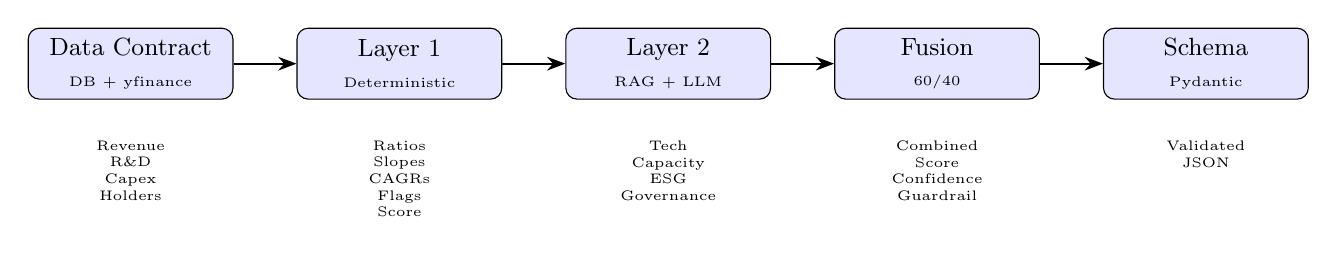
\begin{tikzpicture}[
  node distance=0.5cm and 0.8cm,
  box/.style={draw, rounded corners, fill=blue!10, minimum width=2.6cm,
              minimum height=0.9cm, align=center, font=\small},
  arr/.style={-Stealth, thick}
]

\node[box] (dc)  {Data Contract\\{\tiny DB + yfinance}};
\node[box, right=of dc] (l1)  {Layer 1\\{\tiny Deterministic}};
\node[box, right=of l1] (l2)  {Layer 2\\{\tiny RAG + LLM}};
\node[box, right=of l2] (fu)  {Fusion\\{\tiny 60/40}};
\node[box, right=of fu] (sc)  {Schema\\{\tiny Pydantic}};

\draw[arr] (dc) -- (l1);
\draw[arr] (l1) -- (l2);
\draw[arr] (l2) -- (fu);
\draw[arr] (fu) -- (sc);

\node[below=0.4cm of dc,  font=\tiny, align=center] {Revenue\\R\&D\\Capex\\Holders};
\node[below=0.4cm of l1,  font=\tiny, align=center] {Ratios\\Slopes\\CAGRs\\Flags\\Score};
\node[below=0.4cm of l2,  font=\tiny, align=center] {Tech\\Capacity\\ESG\\Governance};
\node[below=0.4cm of fu,  font=\tiny, align=center] {Combined\\Score\\Confidence\\Guardrail};
\node[below=0.4cm of sc,  font=\tiny, align=center] {Validated\\JSON};

\end{tikzpicture}
\end{center}

\vspace{0.3cm}
\small
\begin{itemize}
  \item \textbf{Data Contract} is the single data boundary --- all downstream code
        touches only \texttt{InputBundle}, never raw DB rows or DataFrames
  \item \textbf{Layer 1} is fully offline-testable: no LLM, no network, pure NumPy
  \item \textbf{Layer 2} runs hybrid retrieval first, then passes evidence + L1 numbers
        to the LLM in a single structured prompt
  \item \textbf{Pydantic schema} validates all fields and range constraints before
        the result is returned
\end{itemize}

\end{frame}

%=========================================================
% SLIDE 15 : END
%=========================================================
\begin{frame}{END}
\Large
\begin{center}
\textbf{Thank You}
\end{center}
\end{frame}

\end{document}
